\documentclass{article} % For LaTeX2e
\usepackage{nips14submit_e,times}
\usepackage{amsmath}
\usepackage{amsthm}
\usepackage{amssymb}
\usepackage{mathtools}
\usepackage{hyperref}
\usepackage{url}
\usepackage{algorithm}
\usepackage[noend]{algpseudocode}
%\documentstyle[nips14submit_09,times,art10]{article} % For LaTeX 2.09

\usepackage{mathrsfs}
\usepackage{graphicx}
\usepackage{caption}
\usepackage{subcaption}

\def\eQb#1\eQe{\begin{eqnarray*}#1\end{eqnarray*}}
\def\eQnb#1\eQne{\begin{eqnarray}#1\end{eqnarray}}
\providecommand{\e}[1]{\ensuremath{\times 10^{#1}}}
\providecommand{\pb}[0]{\pagebreak}


\def\Qb#1\Qe{\begin{question}#1\end{question}}
\def\Sb#1\Se{\begin{solution}#1\end{solution}}

\newenvironment{claim}[1]{\par\noindent\underline{Claim:}\space#1}{}
\newtheoremstyle{quest}{\topsep}{\topsep}{}{}{\bfseries}{}{ }{\thmname{#1}\thmnote{ #3}.}
\theoremstyle{quest}
\newtheorem*{definition}{Definition}
\newtheorem*{theorem}{Theorem}
\newtheorem*{lemma}{Lemma}
\newtheorem*{question}{Question}
\newtheorem*{preposition}{Preposition}
\newtheorem*{exercise}{Exercise}
\newtheorem*{challengeproblem}{Challenge Problem}
\newtheorem*{solution}{Solution}
\newtheorem*{remark}{Remark}
\usepackage{verbatimbox}
\usepackage{listings}

\title{Real Variables: \\
Problem Set X}


\author{
Youngduck Choi \\
Courant Institute of Mathematical Sciences \\
New York University \\
\texttt{yc1104@nyu.edu} \\
}


% The \author macro works with any number of authors. There are two commands
% used to separate the names and addresses of multiple authors: \And and \AND.
%
% Using \And between authors leaves it to \LaTeX{} to determine where to break
% the lines. Using \AND forces a linebreak at that point. So, if \LaTeX{}
% puts 3 of 4 authors names on the first line, and the last on the second
% line, try using \AND instead of \And before the third author name.

\newcommand{\fix}{\marginpar{FIX}}
\newcommand{\new}{\marginpar{NEW}}

\nipsfinalcopy % Uncomment for camera-ready version

\begin{document}


\maketitle

\begin{abstract}
This work contains solutions to the problem set 
X of Real Variables 2015 at NYU.
\end{abstract}

\section{Solutions}

\begin{question}[1. Royden 13-41]
\hfill
\begin{figure}[h!]
  \centering
    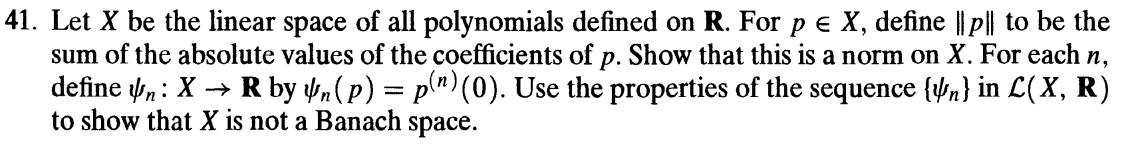
\includegraphics[width=1\textwidth]{13-41.png}
\end{figure}
\end{question}
\begin{solution} We first show that $\lVert \> \rVert:X \to \mathbb{R}$
given is a norm on $X$. First of all, 
\ 
\end{solution}

\newpage

\begin{question}[2. Royden 14-18]
\hfill
\begin{figure}[h!]
  \centering
    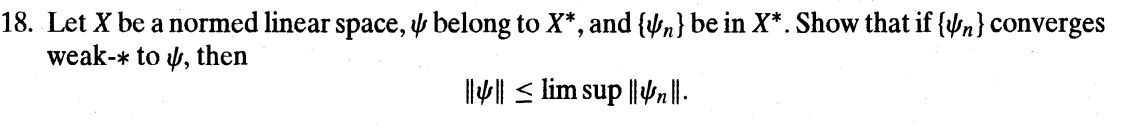
\includegraphics[width=1\textwidth]{14-18.png}
\end{figure}
\end{question}
\begin{solution}
\end{solution}

\newpage

\begin{question}[3. Royden 14-23]
\hfill
\begin{figure}[h!]
  \centering
    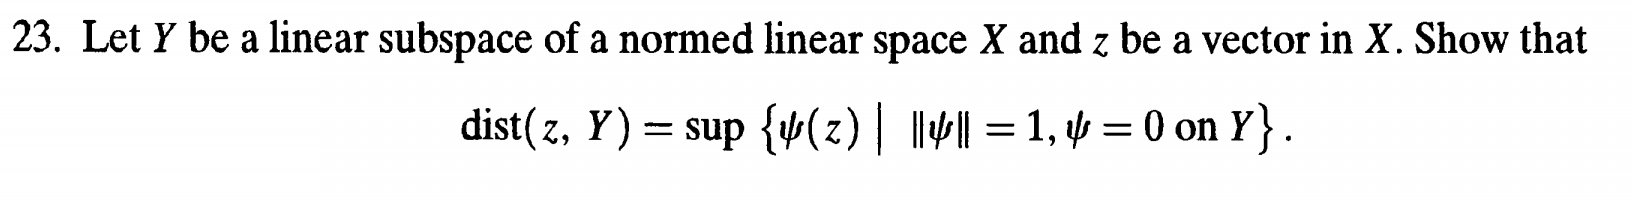
\includegraphics[width=1\textwidth]{14-23.png}
\end{figure}
\end{question}
\begin{solution}
\end{solution}

\newpage

\begin{question}[4. Royden 15-12]
\hfill
\begin{figure}[h!]
  \centering
    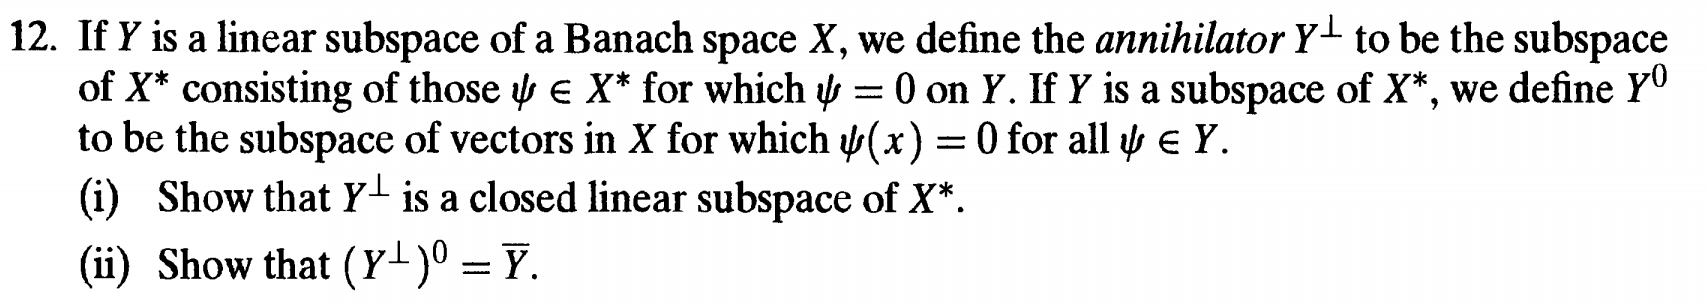
\includegraphics[width=1\textwidth]{15-12.png}
\end{figure}
\end{question}
\begin{solution}
\end{solution}
\end{document}
